\documentclass[12pt]{exam}

% essential packages
\usepackage{fullpage} % margin formatting
\usepackage{enumitem} % configure enumerate and itemize
\usepackage{amsmath, amsfonts, amssymb, mathtools} % math symbols
\usepackage{xcolor, colortbl} % colors, including in tables
\usepackage{makecell} % thicker \Xhline in table
\usepackage{graphicx} % images, resizing

% sometimes needed packages
\usepackage{hyperref} % hyperlinks
% \hypersetup{colorlinks=true, urlcolor=blue}
% \usepackage{logicproof} % natural deduction
\usepackage{tikz} % drawing graphs
\usetikzlibrary{positioning}
% \usepackage{multicol}
% \usepackage{algpseudocode} % pseudocode

% paragraph formatting
\setlength{\parskip}{6pt}
\setlength{\parindent}{0cm}

% newline after Solution:
\renewcommand{\solutiontitle}{\noindent\textbf{Solution:}\par\noindent}

% less space before itemize/enumerate
\setlist{topsep=0pt}

% creates \filcl to grey out cells for groupwork grading
\newcommand{\filcl}{\cellcolor{gray!25}}

% creates \probnum to get the problem number
\newcounter{probnumcount}
\setcounter{probnumcount}{1}
\newcommand{\probnum}{\arabic{probnumcount}. \addtocounter{probnumcount}{1}}

% use roman numerals by default
\setlist[enumerate]{label={(\roman*)}}

% creates custom list environments for grading guidelines, question parts
\newlist{guidelines}{itemize}{1}
\setlist[guidelines]{label={}, left=0pt .. \parindent, nosep}
\newlist{gwguidelines}{enumerate}{1}
\setlist[gwguidelines]{label={(\roman*)}, nosep}
\newlist{qparts}{enumerate}{2}
\setlist[qparts]{label={(\alph*)}}
\newlist{qsubparts}{enumerate}{2}
\setlist[qsubparts]{label={(\roman*)}}
\newlist{stmts}{enumerate}{1}
\setlist[stmts]{label={(\roman*)}, nosep}
\newlist{pflist}{itemize}{4}
\setlist[pflist]{label={$\bullet$}, nosep}
\newlist{enumpflist}{enumerate}{4}
\setlist[enumpflist]{label={(\arabic*)}, nosep}

\printanswers

\begin{document}
%%%%%%%%%%%%%%% TITLE PAGE %%%%%%%%%%%%%%%
\title{EECS 203: Discrete Mathematics\\
  Fall 2023\\
  Homework 5}
\date{}
\author{}
\maketitle
\vspace{-50pt}
\begin{center}
  \huge Due \textbf{Thursday, October. 12}, 10:00 pm\\
\Large No late homework accepted past midnight.\\
\vspace{10pt}
\large Number of Problems: $7+2$
\hspace{3cm}
Total Points: $100+20$
\end{center}
\vspace{25pt}
\begin{itemize}
    \item \textbf{Match your pages!} Your submission time is when you upload the file, so the time you take to match pages doesn't count against you.
    \item Submit this assignment (and any regrade requests later) on Gradescope. 
    \item Justify your answers and show your work (unless a question says otherwise).
    \item By submitting this homework, you agree that you are in compliance with the Engineering Honor Code and the Course Policies for 203, and that you are submitting your own work.
    \item Check the syllabus for full details.
\end{itemize}
\newpage
%%%%%%%%%%%%%%% TITLE PAGE %%%%%%%%%%%%%%% 

\section*{Individual Portion}

\subsection*{\probnum Induction Construction [16 points]} 
Let $P(n)$ be the statement that $1 \cdot 1! + 2 \cdot 2!+\dots+ n \cdot n! = (n + 1)! - 1$
whenever $n$ is a positive integer. In this problem, we will prove this statement via weak induction.
\begin{qparts}
    \item What is the statement $P(1)$?
    \item Show that $P(1)$ is true, which is the base case for our inductive step.
    \item In the base case we prove $P(1)$; what do you need to prove in the inductive step?
    \item What is the inductive hypothesis for your proof?
    \item Complete the inductive step, indicating where you used the inductive hypothesis.
    \item Explain why this proof shows $P(n)$ is true for all positive integers $n$.
\end{qparts}

\begin{solution}
    \begin{qparts}
        \item $P(1)$: $1 \cdot 1! = (1+1)!  - 1$.
        \item For $P(1)$, LHS =  1\\
                    RHS = $2! - 1 = 2 \cdot 1 - 1 = 1$.\\.
                    $\therefore$ LHS = RHS.
                    $\therefore$ $P(1)$ is true.
        \item We need to prove that $P(k) \rightarrow P(k+1)$ for any integer $n$ which is $\geq$ 1.
        \item The inductive hypothesis: Assume $P(k)$: $1 \cdot 1! + 2 \cdot 2!+\dots+ n \cdot n! = (n + 1)! - 1$.
        \item Let $k$ be an arbitrary positive integer.\\
            Assume $P(k)$: $1 \cdot 1! + 2 \cdot 2!+\dots+ n \cdot n! = (n + 1)! - 1$\\
            Want to show: $P(k+1)$: $1 \cdot 1! + 2 \cdot 2!+\dots+ n \cdot n! + (n+1) \cdot (n+1)! = (n + 1 + 1)! - 1$\\
            Using $P(n)$ we know: 
            \begin{align*}
                1 \cdot 1! + 2 \cdot 2!+\dots+ n \cdot n! + (n+1) \cdot (n+1)! &= (n + 1)! - 1 + (n+1) \cdot (n + 1)! \\
                &= (n+1)! (1 + n + 1) + 1\\
                &= (n + 1 + 1)\cdot (n+1) \cdot n \cdot (n-1) \cdot \cdots \cdot 1 -1\\
                &= (n + 1 + 1)! -1
            \end{align*}
            Thus $P(k) \rightarrow P(k+1)$ for any integer $n$ which is $\geq$ 1.
        \item It is because that: (1) $P(1)$: $1 \cdot 1! = (1+1)!  - 1$.\\
            (2)$P(k) \rightarrow P(k+1)$ for any integer $n$ which is $\geq$ 1.\\
            Therefore $P(1) \rightarrow P(2) \rightarrow P(3) \cdots \rightarrow P(n)$\\
            Where $n$ can be any positive integer.\\
            $\therefore$ Since we know (1) is true and (2) is true, $P(n)$ is true for all positive integers $n$.

    \end{qparts}
\end{solution}


\subsection*{\probnum Base Two Blues [14 points]}
Prove using mathematical induction that $\text{log}_2 (n) < n$ for every positive integer $n$. You may assume that the base-2 logarithm function is strictly increasing on its domain.

\textbf{Fun Fact:} $\text{log}_b(n) < n$ is actually true for every positive real number $n$ and arbitrary base $b>1$, but we're asking you to prove this by induction for the special case where $b =2$ and $n$ is a positive integer.

\begin{solution}
    Let $k$ be an arbitrary positive integer.\\
    Assume $P(k)$: $\log_2{k} < k$\\
    Want to show: $P(k+1):$ $\log_2{k+1} < k + 1$\\\\
    \textbf{Base Case:}\\
    $P(0): \log_2{1} < 1$ \\
    Since $\log_2{1} = 0 < 1$, base case is true.\\\\
    \textbf{Inductive Step:}\\
    Using the property of logarithm we know:
    \begin{align*}
        \log_2{(k+1)} &= \log_2{(\frac{k+1}{k} \cdot k)}\\
                    &= \log_2{\frac{k+1}{k}} + \log_2{ k}\\
                    &= \log_2{(1 + \frac{1}{k})} + \log_2{ k}
    \end{align*}
    Since $k$ is a positive integer, $k \geq 1$, $\frac{1}{k} \leq 1$, $\frac{1}{k} + 1\leq 2$\\
    $\therefore \log_2{(\frac{1}{k} + 1)} \leq 1$. \\
    Using $P(n)$ we know: $\log_2{k} < k$. \\
    And Since $\log_2{(\frac{1}{k} + 1)} \leq 1$ and $\log_2{k} < k$\\
    $log_2{(k+1)} = \log_2{(1 + \frac{1}{k})} + \log_2{ k} < k + 1$.\\
    Then we have proved that $P(K) \rightarrow P(k+1)$ for all positive integer $k$.\\\\
    Conclusion: $\text{log}_2 (n) < n$ for every positive integer $n$.
\end{solution}


\subsection*{\probnum Inductive Hypothe-six [15 points]}
Prove by weak induction that 6 divides $n^3 - n$ where $n$ is a nonnegative integer. Don't include unneeded base cases.

\begin{solution} 
    Let $k$ be an arbitrary nonnegative integer.\\
    Assume $P(k)$: $6 | (k^3 - k)$\\
    Want to show: $P(k+1)$: $6 | [(k+1)^3 - (k+1)]$\\\\
    \textbf{Base Case:}\\
    $P(0)$: $6 | 0^3 - 0$\\
    Since $0^3 - 0 = 0$, $6 | 0$, base case is true.\\\\
    \textbf{Inductive Step:}\\
    Since $P(k)$: $6 | (k^3 - k)$, for some integer $m$, $6m = (k^3 - k)$\\
    Then 
    \begin{align*}
        (k+1)^3 - (k+1) &= k^3 + 3k^2 + 3k + 1 - k - 1 \\
                        &= k^3 + 3k^2 + 2k \\
                        &= (k^3 - k) + 3k^2 + 3k \\
                        &= 6m + 3(k^2 + k)
                        &= 6m + 3k\cdot(k+1)
    \end{align*}
    Since $k$ is an integer, and integers consist of alternating odd numbers and even numbers, 
    one of $k$ and $k+1$ must be even. WLOG assume $k$ is even, then for some integer $p$, $k=2p$. \\
    Then $(k+1)^3 - (k+1) = 6m + 3 \cdot 2p\cdot(k+1) = 6m + 6p\cdot (k + 1) = 6[m + p(k+1)]$\\
    Since $p,m,k$ are integers, $p(k+1)$ is an integer, $[m + p(k+1)]$ is an integer.\\
    Then $6 | [m + p(k+1)]$, i.e. $6 | [(k+1)^3 - (k+1)]$. \\
    Therefore we have proved that $P(k) \rightarrow P(k+1)$ for any nonnegative integer $k$.\\\\
    Conclusion: 6 divides $n^3 - n$ where $n$ is a nonnegative integer.
\end{solution}


\subsection*{\probnum Incorrect Strong Induction [14 points]}
For each of the following \textbf{incorrect} strong induction proofs, note where the strong induction proof breaks down and is incorrect.

\textbf{Hint:} Consider where the inductive step breaks down.

\begin{qparts}
    \item Proving for every nonnegative integer $n$, $P(n)\colon 3n = 0$.
    
    \textbf{Inductive Step:}
    
    Assume that $P(j)\colon 3j = 0$ for all nonnegative integers $j$ with $0 \leq j \leq k$. We wish to show $P(k+1)$. We will rewrite $k+1 = a + b$ where $a$ and $b$ are nonnegative integers less than $k+1$. Thus, $3 \cdot (k+1) = 3 \cdot (a+b) = 3a + 3b = 0 + 0 = 0$, therefore $P(k+1)$ is proven.
    
    \textbf{Base Case:} $P(0)\colon 3 \cdot 0 = 0$
    
    Since we have shown the basis step and the inductive step, we have proved for every nonnegative integer $n$, $P(n): 3n = 0$.
    
    \item Proving that every cent value above 3 cents can be formed using just 3-cent and 4-cent stamps.
    
    \textbf{Inductive Step:}
    
    Assume we can form cent values of $j$ cents for all $3 \leq j \leq k$ using just 3-cent and 4-cent stamps. We wish to show we can form $k+1$ cents using just 3-cent and 4-cent stamps. We can form a $k+1$ cent value by replacing 1 3-cent stamp with 1 4-cent stamp or by replacing 2 4-cent stamps with 3 3-cent stamps.
    
    \textbf{Base Case:}
    
    We can form cent values of 3-cents using one 3-cent stamp and we can form cent values of 4-cents using one 4-cent stamp. This covers our two base cases.
    
    Since we have shown the basis step and the inductive step, we have proved every cent value above 3 cents can be formed using just 3-cent and 4-cent stamps.
\end{qparts}

\begin{solution}
    \begin{qparts}
        \item 
            The proof breaks down from the base case when we induce $P(0) \rightarrow P(1)$.\\
            At this point, $k + 1 = 1$, but we cannot find 
            two integers $a$ and $b$ that are less than 1 while they add up to 1.If $a$, $b$ are less than 1 and nonnegative, 
            then they can only be both 0. Then they add to to 0 but not 1.\\
            Therefore the proof is incorrect.

        \item 
            The proof breaks down when we induce $(P(3) \land P(4)) \rightarrow P(5)$.\\
            The inductive step states that we can form a $k + 1$ cent value by 
            replacing 1 3-cent stamp with 1 4-cent or by replacing 2 4-cent stamps with 3 3-cent stam. 
            But at this point, we only have one 4-cent and can not apply the induction.\\
            Therefore the proof is incorrect.
            
    \end{qparts}
\end{solution}


\subsection*{\probnum Chopping Ice [15 points]}
Claire doesn't have an ice tray, so she makes ice by freezing water into a rectangle and then dividing the rectangle into grid-aligned cells. She would like to divide her block of ice into $n$ rows and $m$ columns quickly, before the ice melts! See the image below for an example.
\begin{center}
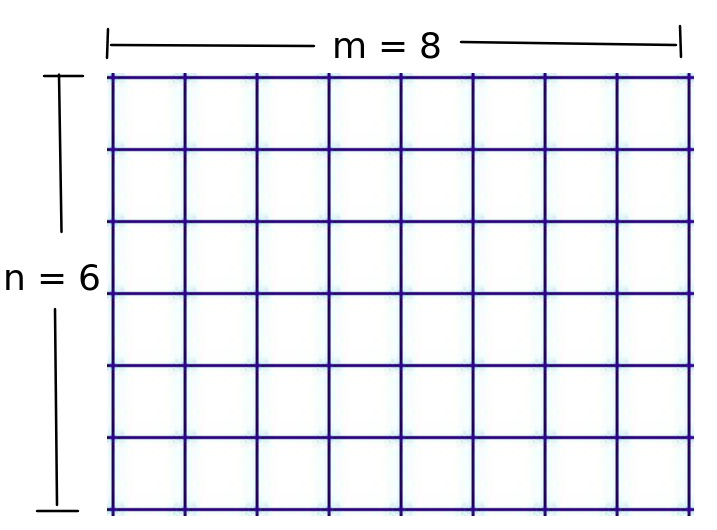
\includegraphics[scale = 0.3]{ice.png}
\end{center}
\begin{qparts}
    \item State the number of cuts Claire needs to make to divide her ice block into $n \times m$ cells. One cut means splitting a single rectangle into two rectangles. In other words, you may NOT make a single cut across multiple pieces of ice. You may use $n$ and/or $m$ in your answer.
    
    \item Prove your answer from part (a).
\end{qparts}

\begin{solution} 
    \begin{qparts}
        \item $(n-1) + n\cdot (m-1) = mn - 1$\\
             $m,n$ are positive integers.
        \item 
        Let $m,n$ be an arbitrary positive integer. $k(m,n)$ is 
        the number of cuts to make to divide her ice block into $n \times m$ cells.\\
        Assume $P(m,n)$: $k(m,n) = mn - 1$\\
        WLOG (due to symmetry, $k(m+1, n ) = k(m,n+1)$), 
        we want to show: $P(m, n+ 1)$: $k(m,n + 1) = m(n+1) - 1$\\\\

        \textbf{Inductive Step:}\\
        We can first cut the (n+1) row from the block. This requires 1 cut.\\
        Then we get $n \times m$ block and $1\times m$ block.\\
        \begin{center}
            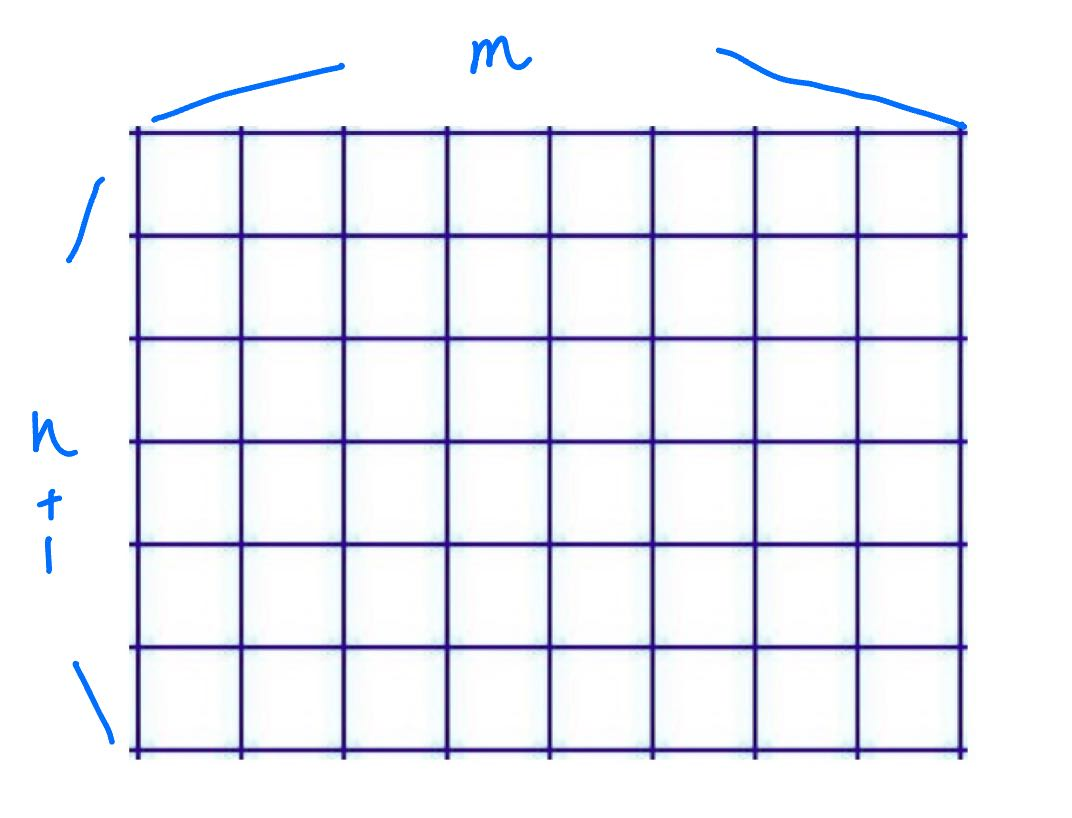
\includegraphics[scale = 0.15]{WechatIMG676.jpeg}\\
            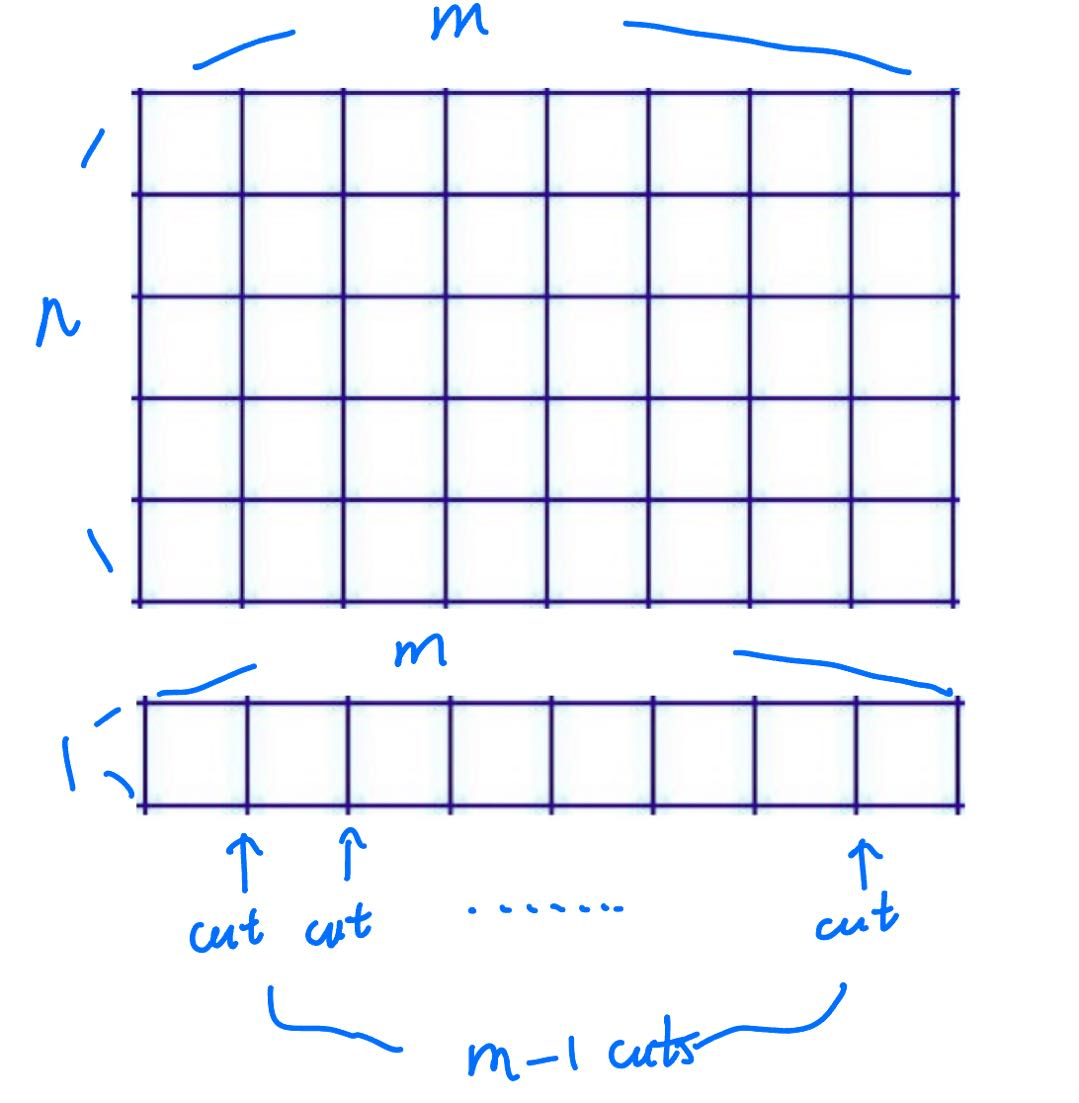
\includegraphics[scale = 0.15]{WechatIMG675.jpeg}\\
        \end{center}
        From the inductive hypothesis we know, to divide the $n \times m$ block, we need $k(m,n)$ cuts.\\
        And to divide the $1 \times m$ block, since we can not make 
        a single cut across multiple pieces of ice, we can only use $m-1$ cuts.\\
        $\therefore$ In total, we need:
        \begin{align*}
            1 + k(m,n) + (m-1) &= 1 + mn - 1 + m - 1\\
                           &= mn + m - 1\\
                           &= m(n + 1) - 1
        \end{align*}
        
        
        \textbf{Base Case:} 
        To divide a 
        $P(1,1): k(1,1) = 1 \times 1 - 1 = 0$ is true.\\

        Since $P(1,1)$, $P(m,n) \rightarrow P(m, n+1)$, and due to symmetry $P(m,n) \rightarrow P(m+1, n)$,
        $P(m,n)$ is true for any positive integer $m,n$.

        Conclusion: We need $mn -1$ cuts to divide her ice block into $m\times n $ cells.

    \end{qparts}

\end{solution}


\subsection*{\probnum Pastry Recurrence [12 points]}
A baker decorates a cookie in 2 minutes, a cupcake in 3 minutes, and a pie in 3 minutes.
Let $a_n$ denote the number of distinct ways the baker decorates pastries in exactly $n$ minutes for $n \geq 0$ (where order matters).
\begin{qparts}
    \item Find a recurrence relation for $a_n$.
    \item What are the initial conditions? Use the fewest initial conditions necessary. 
\end{qparts}

\begin{solution}
    \begin{qparts}
        \item 
        Case 1: The last pastry the baker decoratess is cookie.\\
            Then before that, there are $a_{n-2}$ ways.\\
        Case 2: The last pastry the baker decorates is cupcake.\\
            Then before that, there are $a_{n-3}$ ways.\\
        Case 3: The last pastry the baker decorates is pie.\\
            Then before that, there are $a_{n-3}$ ways.\\
        $\therefore$ $a_n = a_{n-2} + 2 a_{n-3}$. ($n \geq 3$)
        \item 
        Since $a_n$ is valid only when $n \geq 0$, and we have $a_{n-3}$ in our recurrence relation,
         we need to know all $a_n$ where $n < 3$.\\
         That is: \\
        $a_0 = 1$ (since the only choice is to do nothing)\\
        $a_1 = 1$ (since the only choice is to do nothing)\\
        $a_2 = 1$ (since the only choice is to decorate a cookie.)
    \end{qparts}

\end{solution}


\subsection*{\probnum Raven's Wrestlers [14 points]}
Raven has $n$ weeks to build her wrestling figure collection.  Every week, Raven buys one item to add to her collection.  There are 4 different types of things she can buy: Figures, T-shirts for her wrestlers to wear, Weapons for them to fight with, or Display Stands to show them off on her shelves.
\begin{itemize}
    \item Her shelves can fit 2 Stands nicely, so when she buys a Display Stand, she will always buy a second one the next week to finish the shelf.  Additionally, the week after buying the second Stand, she will buy something other than a Display Stand (they aren't as exciting to buy)
    \item When she buys a Figure, she gets very excited about it and wants to buy a new T-shirt for it to wear the following week.
\end{itemize}
Let $a_n$ represent the number of ways Raven can buy items across the $n$ weeks (where $n\geq 0$)
\begin{qparts}
    \item Find a recurrence relation for $a_n$.
    \item Which terms would need to be defined with initial conditions (no need to find the value, just which terms)
\end{qparts}
\textit{Note 1:} Buying the same items in a different order counts as a different way of buying items.  We treat all items in a category as identical.

\textit{Note 2:} on week $n$, Raven will not buy a Figure (because she knows she will miss buying a T-shirt) or a Stand (what a sad way to end the collection).  This information is not needed for the simplest solutions, but some alternate solutions may need to know this.

\begin{solution}
    \begin{qparts}
        \item 
        The recurrence relation is:\\
        $$
        a_n = 2a_{n-1} + a_{n-2} + 2a_{n-3} + a_{n-4}
        $$
        \begin{center}
            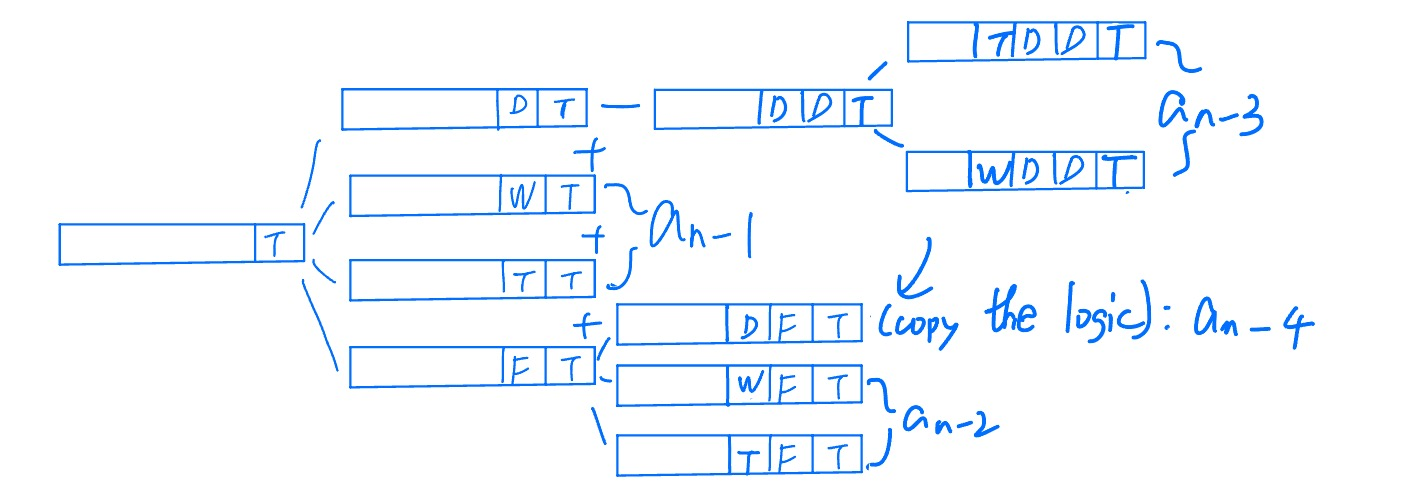
\includegraphics[scale = 0.3]{461697142928_.pic.jpg}\\
            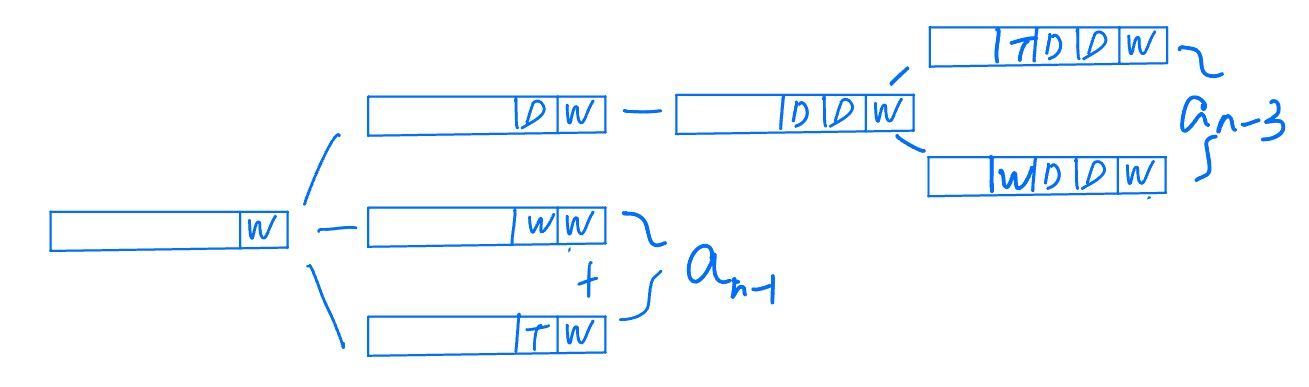
\includegraphics[scale = 0.3]{471697142928_.pic.jpg}\\
        \end{center}
        The logic is shown in the picture.\\
        We use T,W,D,F to indicate the four items.\\
        There are two cases for item in week $n$: T and W.\\
        For the case W in week $n$, there are three possible choices in week $n-1$: D, W, T.
        Number of ways ended with W and T are exactly $a_{n-1}$. And for the way ended with $DW$, the previous
        item can only be D, and therefore get TDDW and WDDW. The number of them are exactly $a_{n-3}$. \\
        \\
        For the case T in week $n$, there are four possible choices in week $n-1$: D, W, T, F. Number of ways ended with WT and TT 
        is exactly $a_{n-1}$, and for FT, the possible choices in week $n-2$ is D,W,T. Number of ways 
        ended with WFT and TFT are exactly $a_{n-2}$.\\
        And for the remaining circumstances DT and DFT beginning with D, 
        we can apply the same logic in the DW case, and get $a_{n-3}$ and $a_{n-4}$ respectively.
        \item 
        since for $a_n$, $n \geq 0 $, and there is $a_{n-4}$ in our recurrence relation, 
        $n - 4 \geq 0$. So the weeks where $n < 4$ should be set as initial conditions.\\
        Therefore $a_1, \, a_2, \, a_3, \, a_4$ would need to be defined with initial conditions.
    \end{qparts}
\end{solution}


\pagebreak

\setcounter{probnumcount}{1}
\section*{Groupwork}
\subsection*{\probnum Grade Groupwork 4}
Using the solutions and Grading Guidelines, grade your Groupwork 4:
\begin{itemize}
    \item Mark up your past groupwork and submit it with this one.
    \item Write whether your submission achieved each rubric item. If it didn't achieve one, say why not.
    \item Use the table below to calculate scores.
    \item For extra credit, write positive comment(s) about your work.
    \item You don't have to redo problems correctly, but it is recommended!
    \item What if my group changed? \begin{itemize}
        \item If your current group submitted the same groupwork last time, grade it together.
        \item  If not, grade your version, which means submitting this groupwork assignment separately. You may discuss grading together.
    \end{itemize}
\end{itemize}

\begin{center}
\resizebox{\textwidth}{!}{\begin{tabular}{| c | c | c | c | c | c | c | c | c | c | c | c | c |}
\hline
 & (i) & (ii) & (iii) & (iv) & (v) & (vi) & (vii) & (viii) & (ix) & (x) & (xi) & Total:\\
\hline
Problem 2 & & & & & &\filcl &\filcl &\filcl &\filcl & \filcl& \filcl& \hspace{1cm}/20\\
\hline 
Problem 3 & & & & & & & &\filcl &\filcl & \filcl& \filcl& \hspace{1cm}/30\\
\Xhline{1.25pt}
Total: &\filcl &\filcl &\filcl &\filcl &\filcl &\filcl &\filcl &\filcl & \filcl& \filcl& \filcl&\hspace{1cm}/50\\
\hline
\end{tabular}}
\end{center}

\subsection*{Previous Group Homework 4(1): Diag Squirrels [20 points]}
Sammy and Sapphire the Diag squirrels are playing a game.
There is a row of $n$ holes, each starting with 203 acorns in it.
They also have a large, unlimited pile of extra acorns.
Sammy and Sapphire take turns, starting with Sammy; when all the holes are empty on
one of the
squirrel's turn, that squirrel loses. On each turn, a squirrel picks a hole,
eats exactly one acorn from it, then places any number of extra acorns they wish
into each hole to the right of that hole.
They may place a different number of acorns into each other hole.
For example, suppose they are playing with $n = 5$ holes and it is Sammy's turn.
Suppose the number of acorns in each hole at the start of Sammy's turn are as
follows.
\begin{center}
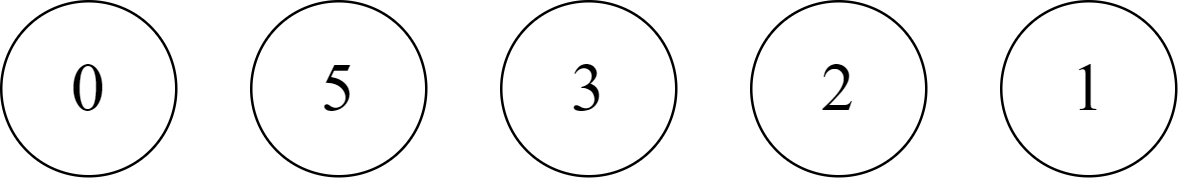
\includegraphics[scale=0.25]{holes1.png}
\end{center}
On their turn, Sammy must pick a hole and eat exactly one acorn from it. Suppose
they pick the third hole. Then the counts become the following:
\begin{center}
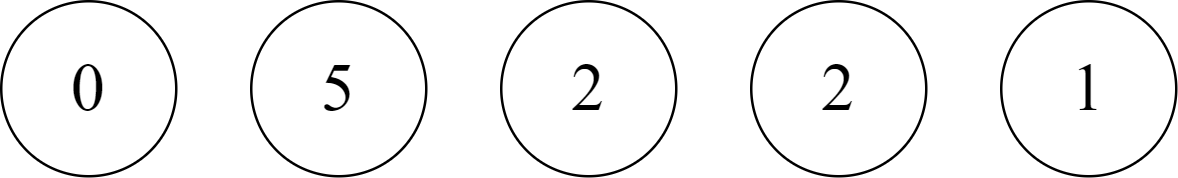
\includegraphics[scale=0.25]{holes2.png}
\end{center}
Sammy may then place any number of extra acorns into each hole to the right of that
hole. In this case, they can place into the fourth and fifth holes. Suppose they
choose to place 3 acorns in the fourth hole and 1 in the fifth. Then the at the end
of Sammy's turn the acorn counts are the following:
\begin{center}
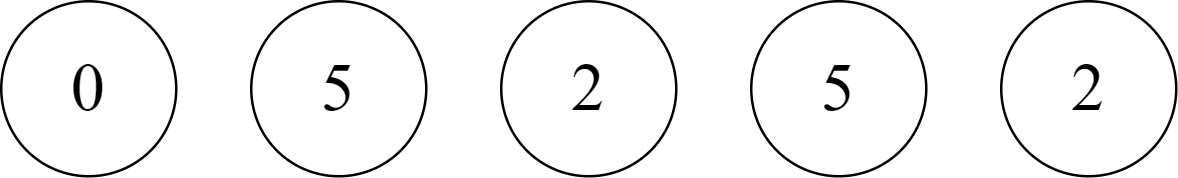
\includegraphics[scale=0.25]{holes3.png}
\end{center}
A winning strategy for a player is a sequence of moves which guarantees that
they will win regardless of what moves their opponent makes. We will construct
a winning strategy for Sammy. We will need an important but non-obvious fact
about this game: the game must reach a state where every hole is
empty except for the right-most hole.
\begin{qparts}
\item Prove that, once we reach the state where all but the right-most hole is
empty,
Sammy has a winning strategy if and only if there are an odd number of acorns
in the hole at the start of their turn.
\item Prove that if a squirrel starts their turn with all holes having an even
number
of acorns (and the game is not over), then at the end of their turn,
at least one hole will have an odd number of acorns.
\item Prove that if a squirrel starts their turn with at least one hole having
an odd number of acorns,
they can end their turn with all holes having an even number of acorns
\item Using the previous parts, prove that Sammy has a winning strategy.
\end{qparts}
\begin{solution}
\begin{qparts}
    \item 
    Let n be an arbitrary integer. There exists n holes.

Case 1: n is odd (there are an odd number of holes)
So there exists an int k such that n = 2k+1.

After turn k:
Sammy will have taken k acorns.
Saph will have taken k acorns.
There will be 2k + 1 - k - k acorns left.
So there will be 1 acorn left.

At turn k+1:
Sammy goes first and eats 1 acorn and ends her turn.
1-1 = 0 acorns left.
Since Saph starts her turn with no acorns, Saph loses and Sammy wins.

Case 2: n is even (there are an even number of holes)
So there exists an int k such that n = 2k.

After turn k:
Sammy will have taken k acorns.
Saph will have taken k acorns.
There will be 2k - k - k acorns left.
So there will be 0 acorns left.

At turn k+1:
Sammy goes first, but there are no acorns left. Sammy loses and Saph wins.

Therefore, Sammy wins if and only if there are an odd \# of acorns at the start of her turn.

\item 
Assume all holes have an even \# of acorns.

So 2a 2b 2c, $2a + 2b + 2c = 2(a+b+c)$
Because $a,b, c$ are ints,$ a+b+c$ is an int. So the total number of acorns is also even.

Let Sammy· take 1 acorn from any hole:
$2(a+b+c) - 1$.
This makes the total number of acorns odd.

Sammy can end her turn without placing any extra acorns, and she will end the turn with at least one hole of odd \# acorns (i.e., the hole that she ate out of). We can prove this statement with a proof by cases: 

If the total number of acorns is odd, then at least one hold is odd.
\begin{enumerate}
    \item Case 1: One hold is odd (then statement proved)
    \item Case 2: No holes are odd. Equivalent to all holes are even. Then total number of acorns will be even: $2(a+b+c…d)$.\\
    This contradicts the assumption
\end{enumerate}

\item 
Assume there is at least one hole with an odd \# of acorns.\\
Let Sammy select the leftmost hole that contains an odd \# of acorns.\\
2n+ 1 2o+1 2p+1 2r+1\\
Sammy chooses 2n+1 hole.

Sammy eats one acorn from that hole, making it even.\\ 
then $2(n), 2o+1, 2p+1,\cdots,2r+1$

Sammy can then place 1 acorn into each of the other odd holes, also making them even. \\
then $2(n), 2o+2, 2p+2, ... ,2r+2$\\
$2(n), 2(o+1), 2(p+1), ... ,2(r+1)$
\\Because Sammy started at the leftmost hole, all odd holes will be accounted for. \\
Thus Sammy always has a way to end the turn with all holes having an even number.

\item  
Given: n holes with 203 holes each.\\
WLOG (regardless if n is odd or even):\\
From c, we know that if Sammy starts w/ at least one odd hole, they can end their turn with all holes having an even \# of acorns. Because all n holes have 203 acorns, there will always be at least one odd hole.\\
Therefore, Sammy can eat an acorn and end her turn in such a way that there will always be all holes with an even \# of acorns.\\
So Sapphire will always start her turn with an even number of acorns.\\
From b, we know that Sapphire has to end her turn with at least one hole having an odd number of acorns.\\
We are given that the game must reach a state where every hole is empty except for the right-most hole.\\
Therefore, the above logic can repeat until there is only one acorn in the right-most hole.\\
Following the logic from part b, since there is an odd number of acorns (i.e., 1), it must be Sammy’s turn.\\
On this turn, Sammy will eat the last acorn and end her turn. 
On Sapphire’s turn, there are no acorns so she loses the game.
\\So in all possible scenarios, Sammy has a winning strategy.
\end{qparts}
\end{solution}
\subsection*{Previous Group Homework 4(2): The Third Dimension [30 Points]}
In lecture, we discussed the problem of tiling a chessboard with dominoes of
dimension $2 \times 1$. We also saw that this question can be made more interesting
by changing the shape of the board.
A related idea to tiling is packing. In a packing question, we no longer care that
the board gets completely covered, instead it is enough to show that a certain
number of dominoes can fit on the board. For example, 32 or fewer $1 \times 2$
dominoes can be packed into a $8 \times 8$ chess board, but 33 or more cannot.
In this problem, we will investigate packing dominoes into a three dimensional
``chess board". In particular, we will prove that it is impossible to pack 53 $1\times 1\times 4$ dominoes into a $6\times 6\times 6$ board.
\begin{qparts}
\item As a warm-up, first show that you \textit{can} pack 54 dominoes into the
board provided that you're allowed to break the dominoes in half.
\item We can divide our board evenly into $2\times 2\times 2$ regions. Consider
coloring these regions red and blue in an alternating fashion. We say that each
$1 \times 1 \times 1$ cell of a domino is colored red if it lies in a red region
and colored blue if it lies in a blue region.
For any domino, list all possible colorings of its 4 cells. Conclude that
exactly half of each domino must lie in a red region.
\item Prove that it is impossible to pack 53 dominoes into a $6\times 6\times
6$ board.
\textbf{Hint:} Figure out how many cells of each color there are, and apply
part (b).
\end{qparts}
\begin{solution}
\begin{qparts}
    \item 
    \begin{center}
        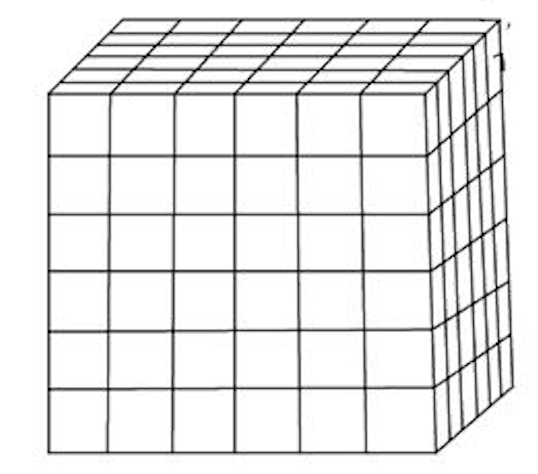
\includegraphics[scale=0.35]{Screenshot 2023-09-28 at 14.26.34.png}
    \end{center}
    
    \begin{center}
        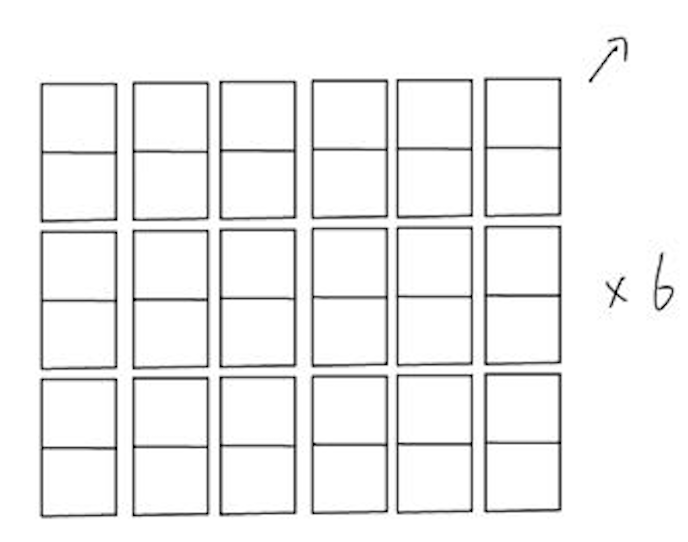
\includegraphics[scale=0.4]{Screenshot 2023-09-28 at 14.26.50.png} 
    \end{center}
    By slicing the cube into 6 identical slices vertically, we have every slice like the picture above. And as we can see, we can fill a slice with $6 \times 3 = 18$ half-dominoes in a slice, and then we fill the 6 identical slices with $18 * 6 = 108$ half-dominoes.
    
    \item 
    \begin{center}
        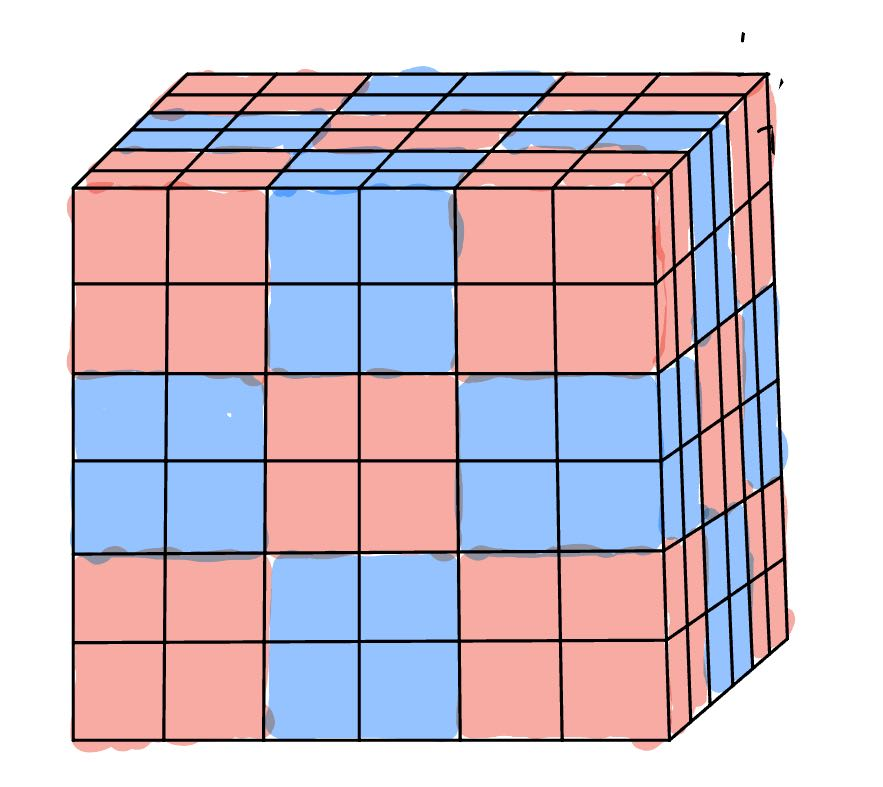
\includegraphics[scale=0.2]{WechatIMG616.jpeg}
    \end{center}
    \begin{center}
        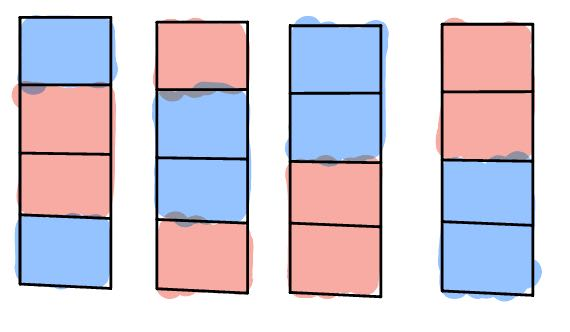
\includegraphics[scale=0.3]{WechatIMG614.jpeg}
    \end{center}
    After we divide the board into $2\times 2\times 2$ regions, if we pack dominoes into the cube board, the 4 possible colorings are as above. We can represent them as BBRR, RRBB, BRRB, RBBR. \\Since every domino contains 2B and 2R, exactly half of each domino must lie in a red region.

    \item 
    After we divide our board into $2 \times 2 \times 2$ regions in alternating color, there should be 27 regions, consisting of 13 blue regions and 14 regions, or 14 blue regions and 13 red regions, dependent on the way we divide.\\
    Since every region contains 8 cells, there would be 8 more blue cells than red cells, or 8 more red cells than blue cells.\\
    Assume that we can pack 53 $1 \times 1 \times 1$ dominoes into the board, then we have $53 \times 2 = 106$ red cells and $53 \times 2 = 106$ blue cells as well.\\
    Then there are $216 - 106 \times 2 = 4$ cells left on the board. Even if they are all red or all blue, that does not meet the quantity. That causes a contradiction.\\
    Therefore we have proved it.
    
\end{qparts}
\end{solution}



\subsection*{\probnum Polly Gone [12 points]}

A convex polygon is a 2D shape with all straight edges such that any line segment between any two non-adjacent vertices passes entirely through its interior (see example picture below). Show via induction that the sum of the interior angles of a convex polygon with $n$ sides is $(n - 2) \cdot 180^{\circ}$. Don't include unneeded base cases.

\begin{center}
    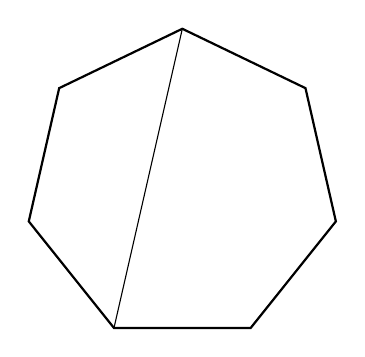
\begin{tikzpicture}[scale = 2]
        \draw[thick, black]  (0,1) -- (0.782,0.623) -- (0.975,-0.223)--(0.434,-0.9)--(-0.434,-0.9)--(-0.975,-0.223)--(-0.782,0.623)--cycle;
        \draw[thin,black] (0,1) -- (-0.434,-0.9);
    \end{tikzpicture}
\end{center}

\textbf{Hint 1}: It is helpful to know that a triangle's interior angles always sum to $180^{\circ}$. You may assume this is true for the problem.

\textbf{Hint 2}: In order to apply your inductive hypothesis to a convex polygon, you'll need to think of it in terms of smaller convex polygons. How can you make smaller polygons out of a big one?

\begin{solution}
    Let $k(n)$ = the sum of the interior angles of a convex polygon with $n$ sides\\
    $P(n): k(n) = (n-2) \cdot 180^{\circ} $\\
    Let $K$ be an arbitrary integer in the domain that $k \geq 4$.\\
    Assume: $P(3) \land P(4) \land P(5) \land ... \land P(k-1)$\\
    Want to prove: $P(k)$
    \\\\
    \textbf{Base Case:}\\
    (Triangle) $n=3$, the sum of the interior angles is $180^\circ $\\
    $k(3) = (3-2) \times 180^\circ  = 1 \times 180^\circ  = 180^\circ $.
    \\\\
    \textbf{Inductive Step:}\\
    Use a straight line to divide the $k$-sides polygon into a triangle and a $(k-1)$-sides polygon.\\
    Using the inductive assumption we know that the $k$-sided polygan should have $(k-2) \times 180^\circ $ degrees for its interior angles.

    Tus the sum of the interior angles is 
    \begin{align*}
        180^\circ  + (k-1-2) \times 180^\circ &= 180^\circ  + (k-3) \times 180^\circ 
                                              &= 180^\circ  \times (1 + k - 3) 
                                              &= 180(k-2)^\circ 
    \end{align*}

    Therefore $P(k)$ is true for every integer $k \geq 4$.
\end{solution}


\smallskip
\subsection*{\probnum Running Recurrence [8 points]}
An EECS 203 student goes to lecture everyday. On each day, she always chooses exactly one method of transportation, and always chooses to walk, bike, or take a bus. She also follows additional rules:
\begin{itemize}
    \item She never walks two days in a row.
    \item If she takes the bus, she must have biked two days ago and walked a day ago.
\end{itemize}

Let $a_n$ denote the number of ways she can go to EECS 203 lecture across $n$ days for $n \geq 0$.
\begin{qparts}
    \item Find a recurrence relation for $a_n$.
    \item What are the initial conditions? Use the fewest initial conditions necessary.
\end{qparts}

\begin{solution}
    \begin{qparts}
        \item The recurrence relation is:
            $$
            a_n = a_{n-1} + a_{n-2} + a_{n-3} + a_{n-4}
            $$
            \begin{center}
                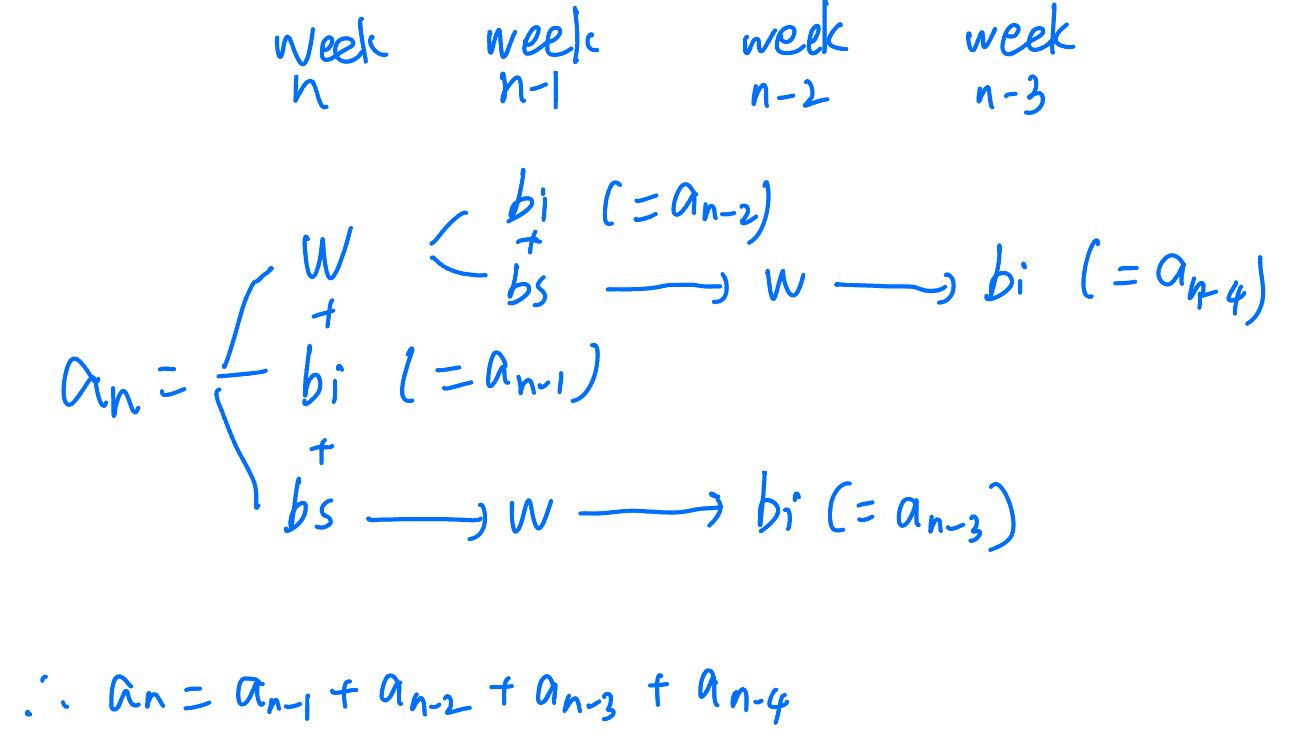
\includegraphics[scale=0.2]{4.jpg}
            \end{center}

            There are 3 cases for the week $n$.\\

            Case 1: In week $n$, she goes to school by bike. This choice has no restrction, so in the weeks before,
            the number of ways she could go to lecture is $a_{n-1}$.
            \\Case 2: In week $n$, she goes to school by bus. This means that in week $n-1$, she walked to school and in
            week $n-2$, she went to lecture by bike. In the weeks before, the number of ways she could go to lecture is $a_{n-3}$.\\
            Case 3: In week $n$, she walks to school. This means that in week $n-1$, she can only went to lecture by bike or by bus. In the
            case she went to lecture by bike, the number of ways she could go to lecture before is $a_{n-2}$. And in the case she wen to 
            lecture by bus, we apply the same logic as in case 2 and get that before the week, the number of ways she could 
            go to lecture is $a_{n-4}$.
        \item
            Since for $a_n$, $n \geq 0$, and in our recurrence relation there is $a_{n-4}$. We need $n-4 \geq 0$ for the 
            recurrence relation. So the cases where $0 \leq n < 4$ should be initial conditions.\\
            That is:
            \\ $a_0 = 1$ (no way)
            \\ $a_1 = 2$ (can only go by bike or on foot)
            \\ $a_2 = 3$ (walk bike, bike walk, bike bike)
            \\ $a_3 = 6$ (walk bike walk, walk bike bike, bike bike walk, bike walk bike, bike bike bike, bike walk bus)

    \end{qparts}
\end{solution}


\end{document}
